% -*-mode: Latex-*-
% !TEX root = thesis.tex
% paper: ...
% authors: simon, raimund
%
% file: block.tex
% contents: permanent blocking analysis
% Sccs-Id: %W% %G%

%------------------------------------------------------------------
%------------------------------------------------------------------

\chapter{Permanent Blocking Analysis of PNSCs with SIAs}
\label{chap_block}
The interaction of concurrent systems in general is fragile in the sense that unwanted blocking can occur.
Especially in the domain of critical systems it is important to ensure that a system is free of permanent blocking.
In \Chap{\ref{chap_tcm}} I introduced a mechanism that allows to punctually remove communication coupling in synchronisation.
In a system where all coupling in synchronisation is removed, no possibility of permanent blocking can occur.
An example of this is a system which follows the \gls{tta}~\cite{kopetz2011c} design principles.
However, as outlined in the previous chapters, in order to allow event-triggered systems (\ie systems with communication coupling) and time-triggered systems to coexist or interact with each other, it must be possible to check that the processes, relying on an event-triggered communication scheme, are free of permanent blocking situations.

In this chapter, I present an analysis to detect permanent blocking in systems of concurrent processes where the interaction is based on synchronous communication, \ie communication with synchronisation coupling.
Based on the semantics of \glspl{sia} I define the meaning of permanent blocking between two or more concurrent processes.
I categorise two possible types of permanent blocking as either {\em lonely blocking} or {\em deadlocks} and present an analysis that is able to identify both types of permanent blocking between two or more concurrent processes.
% This blocking analysis is modular, as it allows to merge two processes by folding their \glspl{sia}, which can be incrementally applied in an arbitrary order to detect lonely blocking and deadlocks between multiple processes.

The chapter is structured as follows:
In \Sect{\ref{sect_block_perm}} I identify permanent blocking situations in \glspl{sia} and propose an analysis to detect permanent blocking states in \Sect{\ref{sect_block_analysis}}.
In \Sect{\ref{sect_block_dl}} I discuss how a subtype of permanent blocking, namely deadlocks, can be identified and propose an analysis to achieve this.
For reasons of simplicity and readability I first focus on permanent blocking and deadlock situations in systems of two concurrent processes.
Later, the findings are extended to hold for the general case.
In \Sect{\ref{sect_block_impl}} I propose an algorithm that allows to compute permanent blocking states and an algorithm to distinguish between permanent blocking and deadlock situations.
% In \Sect{\ref{sect_cci_decoupling}} I introduce communication buffers that allow to decouple process communication in multiple dimensions and, therefore, make the model suitable for mixed-criticality \gls{cps}.
\Sect{\ref{sect_block_summary}} summarises the chapter.

%==============================================================================
\section{Permanent Blocking of SIAs}
\label{sect_block_perm}
In this section I will discuss how a process $M$ can become permanently blocked in a \gls{pnsc} $\mathit{MN}$ by analysing the \gls{sia} $\descSIA{M}$ of process $M$ in the context of \gls{sia} $\descSIA{\mathit{MN}}$ of \gls{pnsc} $\mathit{MN}$.
% We call a \gls{pnsc} $N$ the \emph{context} of a process $P$ if \Def{\ref{def.context.process}} holds and a \gls{sia} $\descSIA{N}$ the \emph{context} of a \gls{sia} $\descSIA{P}$ \Def{\ref{def.context.sia}} holds.
I call a \gls{pnsc} $\mathit{MN}$ the \emph{context} of a process $M$ if \Def{\ref{def_context_process}} holds and a \gls{sia} $\descSIA{\mathit{MN}}$ the \emph{context} of a \gls{sia} $\descSIA{N}$ if \Def{\ref{def_context_sia}} holds.
% Throughout this chapter we use the term \emph{context}  as defined in \Def{\ref{def.context}}.
\begin{definition}[Context of a process]
    \label{def_context_process}
    Let $S_{\mathit{MN}}$ be the set of all processes in a \gls{pnsc} $\mathit{MN}$.
    Then $\mathit{MN}$ is the context of a process $M$ iff $M \in S_{\mathit{MN}}$.
\end{definition}
\begin{definition}[Context of a SIA]
    \label{def_context_sia}
    \Gls{sia} $\descSIA{\mathit{MN}}$ is the context of \gls{sia} $\descSIA{M}$ iff the \gls{pnsc} $\mathit{MN}$ is the context of process $M$ where $\descSIA{\mathit{MN}}$ is the \gls{sia} of $\mathit{MN}$ and $\descSIA{M}$ is the \gls{sia} of $M$.
\end{definition}

% In this section we will discuss how a configuration can lead to a situation where a \gls{sia} resides in a blocking state indefinitely and, consequently, permanently blocks the \gls{pnsc} (or a subsystem of the \gls{pnsc}).
In order to talk about permanent blocking of a \gls{pnsc} we need to establish an understanding of what permanent blocking means.
As defined in \Equ{\ref{eq_liveness}}, we use the term \emph{permanent blocking} as the opposite of \emph{liveness}.
Liveness of a \gls{pnsc} is defined by \Def{\ref{def_liveness_sia_state}, \ref{def_liveness_sia}, \ref{def_liveness_process}, and \ref{def_liveness}}.

\begin{definition}[Liveness of a SIA state]
    \label{def_liveness_sia_state}
    A \gls{sia} $\descSIA{M}$ with context $\descSIA{\mathit{MN}}$ is alive in a state $s \in S_{\descSIA{\mathit{MN}}}$ with $s=\langle s_m, s_n\rangle$ and $s_m \in S_{\descSIA{M}}$, if either
    \begin{enumerate}
    \item[a)] $s_m$ is an end state of $\descSIA{M}$ as defined in \Equ{\ref{eq_sia_end}}, or
    \item[b)] progress is possible from $s$ into a state $s'=\langle s_m', s_n'\rangle$ with $s_m' \in S_{\descSIA{M}}$ and $s_m \neq s_m'$.
    \end{enumerate} 
\end{definition}

\begin{definition}[Liveness of a SIA]
    \label{def_liveness_sia}
    % The liveness of a \gls{sia} $\descSIA{P}$ is defined based on the \gls{sia} $\descSIA{N}$ of its context.
    % , which is the system where $\descSIA{P}$'s process $P$ is part of.
    A \gls{sia} $\descSIA{M}$ is alive in context $\descSIA{\mathit{MN}}$, iff it is alive in all reachable states $s \in S_{\descSIA{\mathit{MN}}}$.
\end{definition}

\begin{definition}[Liveness of a PNSC process]
    \label{def_liveness_process}
    A process $N$ is alive in the context $\mathit{MN}$, iff $\descSIA{M}$ is alive in context $\descSIA{\mathit{MN}}$ where $\descSIA{M}$ is the \gls{sia} of $M$ and $\descSIA{\mathit{MN}}$ is the \gls{sia} of $\mathit{MN}$.
\end{definition}

\begin{definition}[Liveness of a PNSC]
    \label{def_liveness}
    A \gls{pnsc} is alive iff all of its processes are alive.
\end{definition}

%------------------------------------------------------------------------------
\subsection{Permanent Blocking Analysis}
\label{sect_block_analysis}
To perform a permanent blocking analysis I use the composition operation $\otimes$, as defined in \Sect{\ref{sect_sia_composition}}, and provide a formal definition of permanent blocking states in a composed system.
In this dissertation I distinguish between cyclic and acyclic \glspl{sia}.
An acyclic \gls{sia} can be represented by a \gls{dag} whereas a cyclic \gls{sia} cannot.
I first start with a simple analysis where I only consider acyclic \glspl{sia}.
In a second step I extend the analysis by also taking cyclic \glspl{sia} into account.

%------------------------------------------------------------------------------
\subsubsection{Permanent Blocking Analysis with Acyclic SIAs}
\label{sect_block_perm_ac}
In order to verify the liveness conditions of a \gls{sia} $\descSIA{M}$ in its context $\descSIA{\mathit{MN}}$, as defined in \Def{\ref{def_liveness_sia_state}}, I can exploit a property of acyclic \glspl{sia}:
In an acyclic subsystem $\descSIA{M}$ each state with no enabled action is an end state by definition.
As a consequence, when composing two such subsystems with the composition operator $\otimes$, as defined in \Def{\ref{def_sia_comp}}, all states of the composed \gls{sia} where no actions are enabled must be end states in each subsystem.
It follows that in order to check for possible progress (\Def{\ref{def_liveness_sia_state}.b)}) of a subsystem $\descSIA{M}$ in a state $s \in S_{\descSIA{\mathit{MN}}}$ of its context, it is sufficient to check whether state $s$ has enabled actions.
This holds under the assumption that all subsystems in context $\descSIA{\mathit{MN}}$ are acyclic.
Finally, I conclude that a state $s \in S_{\descSIA{\mathit{MN}}}$ is permanent blocking if no actions are enabled in state $s$ and at least one of the two subsystems is not in an end state.

The above conclusion only holds if all involved \glspl{sia} have an end state, which is not necessarily the case for \glspl{sia} with cycles.
Hence, I give a formal definition in \Equ{\ref{eq_sia_block_end}} of the set of permanent blocking states $S_{\descSIA{\mathit{MN}}}^{block-ac}$ of a \gls{pnsc} with two processes $M$ and $N$, assuming both \glspl{sia} $\descSIA{M}$ and $\descSIA{N}$ are described by acyclic graphs (this is denoted by the \emph{-ac} postfix).
The set of end states of a \gls{sia} is defined in \Equ{\ref{eq_sia_end}}.
\begin{equation}
    \label{eq_sia_block_end}
    S_{\descSIA{\mathit{MN}}}^{block-ac} = \Big \{\langle s_m, s_n \rangle \in S_{\descSIA{\mathit{MN}}} \ | \
        \big ( s_m \notin S_{\descSIA{M}}^{end} \lor s_n \notin S_{\descSIA{N}}^{end} \big ) \land \langle s_m, s_n \rangle \in S_{\descSIA{\mathit{MN}}}^{end} \Big \}
\end{equation}

The \gls{sia} $\descSIA{\mathit{MN}}_1$, as depicted in \Fig{\ref{fig_sia_ex_fold}}, is an example of the result of the composition of two acyclic subsystems $\descSIA{M}_2$ and $\descSIA{N}_4$ (see \Fig{\ref{fig_sia_ex}}).
The composed \gls{sia} $\descSIA{\mathit{MN}}_1$ has three states with no enabled actions, namely the states $s_{16}$, $s_{24}$, and $s_{25}$.
The question is whether these states are permanent blocking states or not.
Given that all three states have no enabled actions, it holds that no progress for either subsystem is possible in these states, \ie the liveness condition \Def{\ref{def_liveness_sia_state}.b)} is not satisfied.
Further, I have to check whether the states of both subsystems are end states (\Def{\ref{def_liveness_sia_state}.a)}).
In state $s_{16} \in S_{\descSIA{\mathit{MN}}_1}$ both states in the subsystems, $s_1 \in S_{\descSIA{M}_2}$ and $s_6 \in S_{\descSIA{N}_4}$, are end states as defined in \Equ{\ref{eq_sia_end}}, hence, $s_{16}$ is not a permanent blocking state.
States $s_{24}$ and $s_{25}$, however, are permanent blocking states because, while state $s_2 \in S_{\descSIA{M}_2}$ is an end state, \Equ{\ref{eq_sia_end}} does not hold for states $s_4 \in S_{\descSIA{N}_4}$ and $s_5 \in S_{\descSIA{N}_4}$.
The two states $s_{24}$ and $s_{25}$ represent the situation of the \gls{pnsc} of \Fig{\ref{fig_sia_ex}} where process $M_2$ has concluded its processing (in state $s_2 \in S_{\descSIA{M}_2}$) while process $N_4$ is blocked (either in state $s_4 \in S_{\descSIA{N}_4}$ because the shared action $a$ is never served or in state $s_5 \in S_{\descSIA{N}_4}$ because action $b$ is ignored).

% We observe that in a composition of acyclic \glspl{sia} it is sufficient to 
% the question of whether progress is possible is answered by identifying states with no enabled actions in the composed \gls{sia}.
% Hence, it is sufficient to check wheter 
% Following these observations, we conclude that a state $\langle s_m, s_n, \rangle$ in a \gls{sia} $\descSIA{\mathit{MN}} = \descSIA{M} \otimes \descSIA{N}$ is permanent blocking if no further actions are possible and at least one of the two subsystems is not in an end state.


% In a first attempt we are going to define the set of permanent blocking states of a composed \gls{sia}, described by an acyclic graph.
% The definition of permanent blocking states in a composed \gls{sia} $\descSIA{\mathit{MN}}$, solely based on an end state analysis (the set of end states is defined in \Equ{\ref{eq.sia.end}}), is formally given in \Equ{\ref{eq.sia.block.end}}.
% \begin{multline}
%     \label{eq.sia.block.end}
%     S_{\mathit{FG}}^{block-nc} = \bigg \{\langle s_f, s_g \rangle \in S_{\mathit{FG}} \, | \, ( s_f \notin S_F^{end} \lor s_g \notin S_G^{end} ) \\
%     \land \Big ( \forall s_f' \in S_F, \forall s_g' \in S_G, \forall a \in \mathcal{A}_{\mathit{FG}} \setminus may(\mathcal{A}_{\mathit{FG}}^H) \\ . \ \big \langle \langle s_f, s_g \rangle, a, \langle s_f', s_g' \rangle \big \rangle \notin \delta_{\mathit{FG}} \Big ) \bigg \}
% \end{multline}

% Note that \Equ{\ref{eq.sia.block.end}} only holds for the composition of two subsystems.

% However, the permanent blocking analysis based on the definition of \Equ{\ref{eq.sia.block.end}} is only applicable for \glspl{sia} without cycles because cyclic graphs have, potentially, no end states.
% Because, if the graphs have cycles, and potentially no end states, we are not able to detect permanent blocking
The rationale behind end states is that a process is either in a state where its job is accepted as accomplished or it still has to perform actions in order to accomplish its job and reach an end state.
A process that performs periodic work, which would be represented by a cyclic \gls{sia}, will never reach an end state.
If processes with cyclic \glspl{sia} are composed, it can happen that only one process is performing actions indefinitely (in a cycle) while the other processes are blocked.
There are two different cases where a permanent blocking analysis based on the definition of \Equ{\ref{eq_sia_block_end}} falls short for systems with cyclic \glspl{sia}.
I illustrate this with the help of the \gls{pnsc} depicted in \Fig{\ref{fig_pnsc_cycles}}.
%------------------------------------------------------------------
\begin{figure}[bht]
    \TopFigSpace
    \centering
    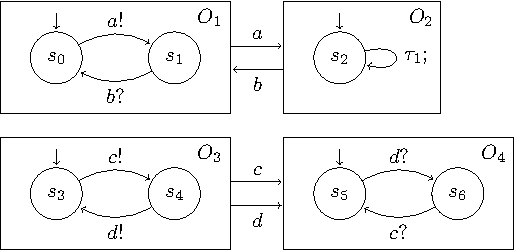
\includegraphics[width=10cm]{fig/sia_pnsc_cycles.pdf}
    \CaptionFigSpace
    \caption{A \gls{pnsc} formed of four processes, each described by a \gls{sia} with a cycle.}
    \label{fig_pnsc_cycles}
    \BotFigSpace
\end{figure}
%------------------------------------------------------------------

The first case is the problem of detecting a lonely blocker when cycles are involved.
This becomes apparent when observing the composed \gls{sia} $\descSIA{O}_{12} = \descSIA{O}_1 \otimes \descSIA{O}_2$:
With the actions $\{a, b\} \in \mathcal{A}_{\descSIA{O}_1}$ ignored, the composed \gls{sia} $\descSIA{O}_{12}$ is formed out of the singe initial state $s_{02}$ with a self looping edge, triggered by the internal action $\tau_1 \in \mathcal{A}_{\descSIA{O}_2}^H$.
In this case the set of permanent blocking states defined in \Equ{\ref{eq_sia_block_end}} is empty because the composed \gls{sia} $\descSIA{O}_{12}$ has no end state.
But clearly, \gls{sia} $O_1$ is permanently blocking in state $s_0$ because the actions $\{a, b\} \in \mathcal{A}_{\descSIA{O}_1}$ are ignored.

The second case is the problem of missing local permanent blocking situations by incrementally folding subsystems of a \gls{pnsc}, depending on the order in which processes are composed.
In the example of \Fig{\ref{fig_pnsc_cycles}}, the \glspl{sia} $\descSIA{O}_3$ and $\descSIA{O}_4$ are both in a permanent blocking state $s_3 \in S_{\descSIA{O}_3}$ and $s_5 \in S_{\descSIA{O}_5}$, respectively.
This is detectable when performing the composition operation $\descSIA{O}_{34} = \descSIA{O}_3 \otimes \descSIA{O}_4$ and computing the set of permanently blocking states as defined in \Equ{\ref{eq_sia_block_end}}.
The composition yields the single initial state $s_{35}$ with no transitions.
Hence, the set of permanent blocking states is defined as $S_{\descSIA{\mathit{O}}_{34}}^{block-ac} = \{ s_{35} \}$, because neither $s_3 \in S_{\descSIA{O}_3}$ nor $s_5 \in S_{\descSIA{O}_4}$ is an end state.
However, when folding the system incrementally, \eg $\descSIA{O}_{1234} = ((\descSIA{O}_1 \otimes \descSIA{O}_2) \otimes \descSIA{O}_3) \otimes \descSIA{O}_4$, the composed \gls{sia} $\descSIA{O}_{1234}$ has no longer an end state and hence, $S_{\descSIA{\mathit{O}}_{1234}}^{block-ac} = \emptyset$.

%------------------------------------------------------------------------------
\subsubsection{Permanent Blocking Analysis with Cyclic SIAs}
\label{sect_block_perm_c}
In the following I extend the previous analysis to work also for cyclic \glspl{sia}.
As defined in \Def{\ref{def_liveness_sia_state}}, in order to decide whether a \gls{sia} $\descSIA{M}$ with context $\descSIA{\mathit{MN}}$ is alive in state $\langle s_m, s_n \rangle \in S_{\descSIA{\mathit{MN}}}$, I need to detect whether \ref{def_liveness_sia_state}.a) $s_m \in S_{\descSIA{M}}$ is an end state of $\descSIA{M}$ or \ref{def_liveness_sia_state}.b) progress from state $\langle s_m, s_n \rangle$ to a state $\langle s'_m, s'_n \rangle$ is possible such that $s_m \neq s'_m$.
I introduce the predicate $progress( sys, s )$, returning true if the latter is true for a subsystem $sys$.
I use this predicate to define the set $\mathit{Sys}_{\descSIA{\mathit{MN}}}(s) \subseteq \{M, N\}$ in \Equ{\ref{eq_sia_sys_alive}} which contains all the subsystems where progress is possible in state $s$ of \gls{sia} $\descSIA{\mathit{MN}}$.
\begin{equation}
    \label{eq_sia_sys_alive}
    Sys_{\descSIA{\mathit{MN}}} \big ( \langle s_m, s_n \rangle \big ) = \Big \{ sys \in \{ M, N \} \ | \ progress \big ( sys, \langle s_m, s_n \rangle \big ) \Big \}
\end{equation}

With the set $\mathit{Sys}_{\descSIA{\mathit{MN}}}(s)$ as defined in \Equ{\ref{eq_sia_sys_alive}} and the set of end states as defined in \Equ{\ref{eq_sia_end}}, in \Equ{\ref{eq_sia_sys}} I define $Sys_{\descSIA{\mathit{MN}}}^{block}\big ( \langle s_m, s_n \rangle \big )$, the set of subsystem identifiers that are permanently blocking in state $\langle s_m, s_n \rangle$ of the composed \gls{sia} $\descSIA{\mathit{MN}}$.
\begin{multline}
    \label{eq_sia_sys}
    Sys_{\descSIA{\mathit{MN}}}^{block}\big ( \langle s_m, s_n \rangle \big ) = \Big \{ M \ | \ s_m \notin S_{\descSIA{M}}^{end} \land M \notin Sys_{\descSIA{\mathit{MN}}} \big (\langle s_m, s_n \rangle \big ) \Big \}
    \\ \cup \ \Big \{ N \ | \ s_n \notin S_{\descSIA{N}}^{end} \land N \notin Sys_{\descSIA{\mathit{MN}}}\big (\langle s_m, s_n \rangle \big ) \Big \}
\end{multline}
Using the set $Sys_{\descSIA{\mathit{MN}}}^{block}\big ( \langle s_m, s_n \rangle \big )$, defined in \Equ{\ref{eq_sia_sys}}, I define the set of permanent blocking states $S_{\descSIA{\mathit{MN}}}^{block}$ of the composed \gls{sia} $\descSIA{\mathit{MN}}$ in \Equ{\ref{eq_sia_block}}.
\begin{equation}
    \label{eq_sia_block}
    S_{\descSIA{\mathit{MN}}}^{block} = \Big \{ \langle s_m, s_n \rangle \in S_{\descSIA{\mathit{MN}}} \ | \ \exists sys \in \{ M, N \} \ . \ sys \in Sys_{\descSIA{\mathit{MN}}}^{block}\big ( \langle s_m, s_n \rangle \big ) \Big \}
\end{equation}
Informally, this means that a state $\langle s_n, s_m \rangle \in S_{\descSIA{\mathit{MN}}}$ is permanently blocking if at least one subsystem is not in an end state and can perform no more actions.

Following \Def{\ref{def_liveness_sia}}, \Def{\ref{def_liveness_process}}, and \Def{\ref{def_liveness}} I can conclude that a \gls{pnsc} composed of the processes $M$ and $N$ is alive if and only if $S_{\descSIA{\mathit{MN}}}^{block} = \emptyset$ with the set $S_{\descSIA{\mathit{MN}}}^{block}$ defined in \Equ{\ref{eq_sia_block}}.

%------------------------------------------------------------------------------
\subsubsection{Permanent Blocking Analysis on an Assembly of Processes}
\label{sect_block_perm_assembly}
In this section I extend the permanent blocking analysis from two subsystems to an arbitrary number of subsystems.
By incrementally applying the folding operation $\otimes$, the initial \gls{pnsc} dependency graph is lost because shared actions are turned to internal actions in the \gls{sia} of the composed process (see \Def{\ref{def_proc_composed}} and \ref{def_sia_comp}).
From a software engineering point of view this might be desirable because it allows to structure big systems hierarchically and allows to reuse code as black boxes where only the interface (specified by a \gls{sia}) is known.
Once a system is composed and guaranteed to be free of permanent blocking, the internal actions can be removed if they do not influence the blocking behaviour of a system.
This can serve to drastically reduce the number of states of the composed system and reduce the behavioural description to the interaction protocol of the composed process.
% However, reducing internal actions is not a simple task because of cycles in the graph and will not be discussed further in this dissertation.
A technique to achieve this is proposed by Pace \etal in~\cite{pace2003} but will not be further discussed in this dissertation.

In order to apply the permanent blocking analysis, described by \Equ{\ref{eq_sia_block}}, to an assembly of incrementally composed processes, two pieces of information must be propagated throughout the process of incrementally folding subsystems with the operator $\otimes$:
First, the dependency graph of the \gls{pnsc} is required in order to retain the dependencies of the subsystems despite the composition.
This preserves the information of which ports are shared by which processes.
Second, a state $s$, of a \gls{sia} composed out of $n$ subsystems, has to be described by the tuple $\langle s_1, \dots, s_n \rangle$ to analyse the permanent blocking state of the initial subsystem and not the incrementally built composition.
These state tuples are extended at each step of the incremental composition by a corresponding state of the subsystem that is composed with the system.

With the propagation of this information, the permanent blocking analysis can be expanded to $n$ subsystems.
Hence, there is no necessity to perform the analysis at each step of the incremental folding operation and can now be applied on the resulting composed system, described by the \gls{sia} $\descSIA{J} = \descSIA{N}_1 \otimes \descSIA{N}_2 \otimes \dots \otimes \descSIA{N}_n$.
Specifically, the set of system identifiers describing subsystems where progress is possible, defined in \Equ{\ref{eq_sia_sys_alive}}, is extended to $n$ subsystems in \Equ{\ref{eq_sia_sys_aliven}}.
\begin{equation}
    \label{eq_sia_sys_aliven}
    Sys_{\descSIA{\mathit{J}}} \big ( \langle s_1, \dots, s_n \rangle \big ) = \Big \{ sys \in \{ N_1, \dots, N_n \} \ | \ progress \big ( sys, \langle s_1, \dots, s_n \rangle \big ) \Big \}
\end{equation}
Similarly, the set of system identifiers describing subsystems that are permanently blocking at a particular state of the composed system, defined in \Equ{\ref{eq_sia_sys}}, is expanded to $n$ subsystems in \Equ{\ref{eq_sia_sysn}}.
\begin{multline}
    \label{eq_sia_sysn}
    Sys_{\descSIA{\mathit{J}}}^{block}\big ( \langle s_1, \dots, s_n \rangle \big ) = \Big \{ N_i \ | \ 1 \leq i \leq n \\
    \land \ s_i \notin S_{\descSIA{N}_i}^{end} \ \land \  N_i \notin \mathit{Sys}_{\descSIA{\mathit{J}}}\big ( \langle s_1, \dots, s_n \rangle \big ) \Big \}
\end{multline}
Finally, the set of permanent blocking states defined in \Equ{\ref{eq_sia_block}} is expanded to $n$ subsystems in \Equ{\ref{eq_sia_blockn}}.
\begin{equation}
    \label{eq_sia_blockn}
    S_{\descSIA{\mathit{J}}}^{block} = \Big \{ \langle s_1, \dots, s_n \rangle \in S_{\descSIA{\mathit{J}}} \ | \ \exists i \in \{ 1, \dots, n \} \ . \  N_i \in \mathit{Sys}_{\descSIA{\mathit{J}}}^{block} \big ( \langle s_1, \dots, s_n \rangle \big ) \Big \}
\end{equation}

The price to pay for propagating state information of subsystems is threefold:
First, the propagation of state information requires an increased memory space as the list of involved subsystems in the state tuple $\langle s_1, \dots, s_n \rangle$ constantly grows.
Second, because permanent blocking situations are not detected when they occur, permanent blocking states are propagated and consequently multiplied.
This leads to an ever growing list of detected permanent blocking situations that may only point to a single cause.
Third, because state information of the subsystems needs to be preserved, it is not directly possible to reduce the state space by reducing internal actions.
However, it is only necessary to preserve the set of subsystem identifiers $\mathit{Sys}(e)$, attributed to each edge representing an internal action, because internal actions cannot cause deadlocks (they are the result of a non-permanent blocking communication).
For example, it should be possible to adopt the reduction technique by Pace \etal~\cite{pace2003} to reduce the data structure used for the analysis.

%------------------------------------------------------------------------------
\subsection{Deadlock Analysis}
\label{sect_block_dl}
In the previous section I established a method to analyse the blocking behaviour of synchronous communication.
In this section I discuss how to distinguish between a \emph{deadlock} of multiple subsystems and \emph{lonely blocking} of a single subsystem.

The crossroad example discussed in \Sect{\ref{sect_ecm_example}} is a typical example of a deadlock situation.
To give an example of a lonely blocker, let's consider the \gls{pnsc} as depicted in \Fig{\ref{fig_sia_lb}}.
The two processes $M_2$ and $N_2$ share the ports $a$ and $b$, and process $M_2$ has a port $c$ that is not (yet) connected to any other process.
Their corresponding \glspl{sia} $\descSIA{M}_2$ and $\descSIA{N}_2$ share the action $a$, action $b \in \mathcal{A}_{\descSIA{N}_2}^O$ is ignored, and action $c \in \mathcal{A}_{\descSIA{M}_2}^I$ is open.
%------------------------------------------------------------------
\begin{figure}[bht]
    \TopFigSpace
    \centering
    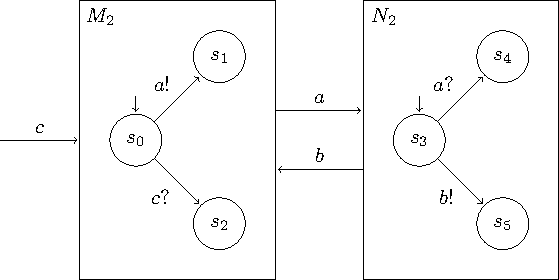
\includegraphics[width=10cm]{fig/sia_lb.pdf}
    \CaptionFigSpace
    \caption{An example of a \gls{pnsc} where the process $M_2$ is alive and process $N_2$ is lonely blocking in state $s_3 \in S_{\descSIA{N}_2}$.}
    \label{fig_sia_lb}
    \BotFigSpace
\end{figure}
%------------------------------------------------------------------

Initially, the two \glspl{sia} start in their respective initial state $s_0$ and $s_3$.
Transitions, labelled by open actions, are assumed to always be triggered by the (unknown) environment.
Hence, \gls{sia} $\descSIA{M}_2$ performs the transition $\langle s_0, c, s_2 \rangle$.
State $s_2$ is, according to \Equ{\ref{eq_sia_end}}, an end state where \gls{sia} $\descSIA{M}_2$ can reside indefinitely.
However, due to the fact that \gls{sia} $\descSIA{M}_2$ has reached an end state and finished its processing, \gls{sia} $\descSIA{N}_2$ will block and wait to synchronize on action $a$ in state $s_3$ indefinitely.
State $s_3$ is not an end state and therefore a permanent blocking state which makes process $N_2$ potentially permanent blocking while process $M_2$ is alive (no permanent blocking states in its corresponding \gls{sia} $\descSIA{M}_2$).
Process $N_2$ is a lonely blocker.

In \Def{\ref{def_dl}} I defined the four conditions that must hold simultaneously for a deadlock to occur.
% Let's apply this to the synchronous communication model as described above.
Condition \ref{enum_mutex} (mutual exclusion) is implicitly satisfied by the produce and consume semantics of the process model.
Condition \ref{enum_preemption} (no pre-emption) must be satisfied by the implementation of the model.
For condition \ref{enum_hold_wait} and \ref{enum_circular} I have to consider the semantics of synchronous communication as it is defined by the model.
Due to the symmetric semantics of synchronous communication, two processes have to be ready simultaneously in order to communicate a message from one to another.
This can be understood as follows:
The receiving process makes a typed buffer available for the sending process to write to.
The sender can only write to the buffer if the type of the message matches.
% The receiver can only make one typed buffer available at a time.
The resources in such a system are the buffers and the message tokens.
If a particular buffer is not available, it is held by the receiver.
If a message token is not currently available for transmission, it is held by the sender.

Applied on the \gls{pnsc} model I observe that the held resources are defined by the signature of a processes, \ie the set of ports.
More precisely, the set of output ports $\mathcal{P}_N^O$ correspond to the typed message tokens held by process $N$ and the set of input ports $\mathcal{P}_N^I$ correspond to the typed buffers held by process $N$.
The type of a buffer or a message token is defined by the name of the corresponding port.
The \gls{sia} of a process in a \gls{pnsc}, on the other hand, defines the required resources by a process.
The resource a process is waiting on depends on the state, the \gls{sia} of the process is currently in.
An input action corresponds to a request for a typed message token and an output action corresponds to a request for a typed buffer.

Formally, I define the predicate $\mathcal{H}(N)$ in \Equ{\ref{eq_hold}}.
It is the set of resources \emph{held} by process $N$ (and its corresponding \gls{sia} $\descSIA{N}$).
\begin{equation}
    \label{eq_hold}
    \mathcal{H}(N) = \mathcal{P}_N^O \cup \mathcal{P}_N^I
\end{equation}
Note that with synchronous communication the set of resources that are held by a process is static and is not depending on the state of the process as it would be the case with asynchronous communication.
Further, I define the predicate $\mathcal{W}(\descSIA{N}, s)$ in \Equ{\ref{eq_wait}}.
It is the set of resources \gls{sia} $\descSIA{N}$ (of process $N$) is \emph{waiting} for in state $s$.
\begin{multline}
    \label{eq_wait}
    \mathcal{W}(\descSIA{N}, s) = \{ a_{buffer} \ | \ \forall d \in \delta_{\descSIA{N}} \ . \ d = \langle s, a, \_ \rangle \ \land \ a \in \mathcal{A}_{\descSIA{N}}^O \} \\
    \cup \{ a_{token} \ | \ \forall d \in \delta_{\descSIA{N}} \ . \ d = \langle s, a, \_ \rangle \ \land \ a \in \mathcal{A}_{\descSIA{N}}^I \} \rangle
\end{multline}

For deadlock condition \ref{enum_hold_wait} (hold and wait) to hold in a particular state $s \in S_{\descSIA{N}}$ of \gls{sia} $\descSIA{N}$ an input or output action must be enabled (an action is enabled if condition defined in \Equ{\ref{eq_sia_enabled}} holds).
Hence, the following condition must be satisfied:
\begin{equation}
    \label{eq_hold_wait}
    \forall s' \in S_{\descSIA{N}}, \exists a \in \mathcal{A}_{\descSIA{N}}^O \cup \mathcal{A}_{\descSIA{N}}^I \ . \ \langle s, a, s' \rangle \in \delta_{\descSIA{N}}
\end{equation}

In order to check whether deadlock condition \ref{enum_circular} (circular wait) is holding, I need to check the wait dependencies of subsystems in permanent blocking states of the composed \gls{sia}.
As the folding operation $\otimes$ is applied incrementally, in an arbitrary order, on each \gls{sia} representing a process in a \gls{pnsc}, I always consider two processes at a time:
The composed process that was constructed out of a subset of the processes of the initial \gls{pnsc} by the incremental folding operation and another process that is not yet incorporated in the composed process but is part of the \gls{pnsc}.
To detect a circular wait of two processes $M$ and $N$ with corresponding \glspl{sia} $\descSIA{M}$ and $\descSIA{N}$ I consider all the permanent blocking states of the composed \gls{sia} $\descSIA{\mathit{MN}}$ and check whether both subsystems are blocked in their corresponding state.
A permanent blocking state $\langle s_m, s_n \rangle \in S_{\descSIA{\mathit{MN}}}$ of \gls{sia} $\descSIA{\mathit{MN}}$ is a deadlock state if the predicate $\mathit{dl}_2(M, N, \langle s_m, s_n \rangle)$, as defined in \Equ{\ref{eq_circular2}}, returns true.
The hold $\mathcal{H}$ and wait $\mathcal{W}$ predicates are defined in \Equ{\ref{eq_hold}} and \Equ{\ref{eq_wait}}, respectively.
% $Sys_{\descSIA{\mathit{MN}}}^{block}(s_m, s_n)$ is defined in \Equ{\ref{eq.sia.sys}}.
% $S_{\mathit{FG}}^{block}(s_f, s_g)$ is computed by replacing line 18 of \Fig{\ref{lst.func.block}} with \texttt{state.blocking.append( sys )} in order to store the name of each blocking subsystem in a list.
% \begin{equation}
%     \label{eq.circular}
% \langle s_m, s_n \rangle \in S_{\descSIA{\mathit{MN}}}^{dl} \, \rightarrow \, (M, N) \in Sys_{\descSIA{\mathit{MN}}}^{block}(s_m, s_n)
% \end{equation}
\begin{equation}
    \label{eq_circular2}
    \mathit{dl}_2(M, N, \langle s_m, s_n \rangle) = \big ( \mathcal{H}(M) \cap \mathcal{W}(\descSIA{N}, s_n) \big) \neq \emptyset \ \land \ \big ( \mathcal{H}(N) \cap \mathcal{W}(\descSIA{M}, s_m) \big ) \neq \emptyset
\end{equation}

% Consequently, subsystem $F$ is lonely blocking in state $s_f$ if $F \in Sys_{\mathit{FG}}^{block}(s_f, s_g) \land G \notin Sys_{\mathit{FG}}^{block}(s_f, s_g)$ and subsystem $G$ is lonely blocking in state $s_g$ if $F \notin Sys_{\mathit{FG}}^{block}(s_f, s_g) \land G \in Sys_{\mathit{FG}}^{block}(s_f, s_g)$.

A circular wait is not necessarily limited to two participants.
More than two processes could be involved in a deadlock.
However, the information of other involved processes that are incorporated in the composed process, is lost due to the incremental folding operation.
In the next section I address this issue.


%------------------------------------------------------------------------------
\subsubsection{Deadlock Analysis on an Assembly of Processes}
\label{sect_block_dl_assembly}

As mentioned before, the deadlock condition \ref{enum_circular} (circular wait) may involve more than two subsystems.
The crossroad example described by \Fig{\ref{fig_cross_proc_sia_dl}} is such a case.
By incrementally folding the processes together, the presented analysis will detect a deadlock at the last step, when folding the system $\descSIA{P}_{\mathit{NW}} \otimes \descSIA{P}_{\mathit{NE}} \otimes \descSIA{P}_{\mathit{SE}}$ with the system $\descSIA{P}_{\mathit{SW}}$.
In reality however, the deadlock is caused by the four individual systems being in a circular wait.

With \Equ{\ref{eq_circular2}} I defined the deadlock condition \ref{enum_circular} (circular wait) for two subsystems $M$ and $N$ in state $\langle s_m, s_n \rangle$.
With the predicate $\mathit{dl}$, as defined in \Equ{\ref{eq_circularn}}, this is expanded to $n$ subsystems.
The ordered set $(N_1, \dots, N_n)$ describes a dependency from subsystem $N_i$ to $N_{i+1}$ and from $N_n$ to $N_1$ to complete the circle.
The state of the composed system is described by the tuple $\langle s_1, \dots, s_n \rangle$, with $s_i$ being a state from the \gls{sia} $\descSIA{N}_i$ of subsystem $N_i$.
\begin{multline}
    \label{eq_circularn}
    \mathit{dl} \big ( (N_1, \dots, N_n), \langle s_1, \dots, s_n \rangle \big ) = \big ( \mathcal{H}(N_n) \cap \mathcal{W}(\descSIA{N}_1, s_1) \big ) \neq \emptyset \\
    \land \ \Big ( \forall N_i | i \in \{1, \dots, n{-}1\}\ .\ \big ( \mathcal{H}(N_i) \cap \mathcal{W}(\descSIA{N}_{i+1}, s_{i+1}) \big ) \neq \emptyset \Big )
\end{multline}

By applying the permanent blocking and deadlock analysis, described in \Sect{\ref{sect_block_perm_assembly}} and this section, respectively, on the example of \Fig{\ref{fig_pnsc_cycles}} in \Sect{\ref{sect_block_perm}} I am now able to identify all cases of permanent blocking and can distinguish between lonely blocking and deadlocks:
Using \Equ{\ref{eq_sia_sys_aliven}}, \Equ{\ref{eq_sia_sysn}}, and \Equ{\ref{eq_sia_blockn}}, I compute the set of permanent blocking states $S_{\descSIA{\mathit{O}}_{1234}}^{block} = \{s_{0235}\}$ and the set of subsystem identifiers $\mathit{Sys}_{\descSIA{O}_{1234}}^{block}(s_{0235}) = \{O_1, O_3, O_4\}$, indicating the permanent blocking subsystems at state $s_{0235}$.
Using the initial dependency graph, $\mathit{Sys}_{\descSIA{O}_{1234}}^{block}(s_{0235})$, and \Equ{\ref{eq_circularn}} I can identify process $O_1$ as lonely blocker, permanently blocking in state $s_0 \in S_{\descSIA{O}_1}$ on action $a \in \mathcal{A}_{\descSIA{O}_1}$.
Further, I find that processes $O_3$ and $O_4$ are in a deadlocking situation, permanently blocking in state $s_3 \in S_{\descSIA{O}_3}$ on action $c \in \mathcal{A}_{\descSIA{O}_3}$ and state $s_5 \in S_{\descSIA{O}_4}$ on action $d \in \mathcal{A}_{\descSIA{O}_4}$, respectively.

%==============================================================================
\section{Implementation of the Permanent Blocking Analysis}
\label{sect_block_impl}
In this section I describe in detail how two aspects of the permanent blocking analysis can be implemented:
First, the computation of the set $\mathit{Sys}_{\descSIA{\mathit{MN}}}(s)$ as defined in \Equ{\ref{eq_sia_sys_aliven}} will be discussed in \Sect{\ref{sect_block_perm_alg}}.
Second, the algorithm to distinguish between lonely blockers and deadlock situation is addressed in \Sect{\ref{sect_block_dl_alg}}.

%------------------------------------------------------------------------------
\subsection{Algorithm to Compute \texorpdfstring{$Sys(s)$}{the Set of Progressing Subsystems}}
\label{sect_block_perm_alg}
While it is fairly simple to compute the set of permanent blocking states of a composed system (as defined in \Equ{\ref{eq_sia_block}}) it is not so trivial to compute the set of subsystems from which progress is possible in a particular state of the composed system (as defined in \Equ{\ref{eq_sia_sys_alive}}).
This is because it is not enough to observe the transitions from one state in order to decide if a subsystem is progressing or not.
A path of successor states and transitions needs to be considered in order to take into account that a subsystem can be temporarily blocked in one state but will still be able to progress in a reachable successor state.
In the following I am going to describe an algorithm that allows to compute the set $\mathit{Sys}(s)$, as defined in \Equ{\ref{eq_sia_sys_alive}}, at each state $s$ of a composed \gls{sia} in linear time complexity.

A straightforward approach to compute $\mathit{Sys}(s)$ is to follow all paths in the composed \gls{sia} and count the involved subsystems along the paths.
% This will allow to identify states that are isolated from subsystems and hence, permanent blocking states.
However, in order to follow all distinct paths in a graph one has to identify all simple cycles in the graph, a problem that is currently known to be solvable in bounded time by $\mathcal{O}\big ( (V+E)(C+1)\big )$~\cite{johnson1975} where $V$ is the number of vertices, $E$ the number of edges, and $C$ the number of cycles in the graph.

Fortunately, I am not explicitly interested in the enumeration of all the paths themselves, but only whether for a state $s$ there exists a path starting with $s$ that includes actions of all subsystems.
%for  but only whether a state is part of a path that involves actions of all subsystems.
This test can be simplified by exploiting the properties of \emph{strongly connected} graphs, \ie graphs where every vertex is reachable from every other vertex in the graph.

For example, if I have a graph component $X$ (\ie a subgraph) in a \gls{sia} that is a strongly connected graph, that means that every state $s \in X$ can reach every state $s' \in X$.
Further, this means that every state $s \in X$ has an outgoing path that includes transitions that are triggered by actions of all the subsystems involved in $X$.
% Therefore, for a permanent blocking analysis, it is sufficient to retain the information of the involved subsystems whereas the information of all possible paths is not required.

From these observations I devise \Alg{\ref{alg_blocking}} to compute the set $Sys(s)$ of subsystems where progress is possible in a particular state $s$ of a composed system.
In the following, the functions, called in each line of \Alg{\ref{alg_blocking}}, are explained in detail.
\begin{figure}[!t]
    \TopAlgSpace
    \removelatexerror
    \begin{algorithm}[H]
        \caption{Permanent Blocking Analysis}
        \label{alg_blocking}
        \begin{algorithmic}[1]
            \Require{\hfill \newline $\descSIA{N}$, the \gls{sia} of a \gls{pnsc} $N$ \newline $s_0$, the initial state of \gls{sia} $\descSIA{N}$}
            \Statex
            \Let{$\langle g_{sia}, v_{init} \rangle$}{$\FuncName{initSiaGraph}( \descSIA{N}, s_0 )$}
            \Let{$Cluster$}{$\FuncName{getConnectedComponents}( g_{sia} )$}
            \Let{$g_{cond}$}{$\FuncName{getClusterGraph}( g_{sia}, Cluster )$}
            \State $\FuncName{propagateSubSys}( g_{cond}, v_{init} )$
            %\State $\FuncName{reassign}( g_{sia}, g_{tree}, cluster, mapping )$
            \State $\FuncName{condensed2Sia}( g_{cond}, g_{sia}, Cluster, \descSIA{N} )$
        \end{algorithmic}
    \end{algorithm}
    \BotAlgSpace
\end{figure}
\begin{description}
    \item[{\normalfont \emph{Line 1:}} Transform a SIA into a Graph] \hfill \\
        $$\langle g_{sia}, v_{init} \rangle \leftarrow \FuncName{initSiaGraph}( \descSIA{N}, s_0 )$$
        The function \texttt{initSiaGraph} takes a \gls{sia} $\descSIA{N}$ and its initial state $s_0$ as input arguments and produces the tuple $\langle g_{sia}, v_{init} \rangle$ as an output.
        A vertex $v$ of the graph $g_{sia}$ corresponds to a state $s \in S_{\descSIA{N}}$.
        I write $v \equiv s$ to indicate the correspondence.
        A directed edge $e$ is defined by a sequence of two vertices, written as $(v_1, v_2)$, where vertex $v_2$ is a direct successor of vertex $v_1$.
        An edge $e = (v_1, v_2)$ of the graph $g_{sia}$ corresponds to a transition $\langle s_1, -, s_2 \rangle \in \delta_{\descSIA{N}}$ where $v_1 \equiv s_1 \in S_{\descSIA{N}}$ and $v_2 \equiv s_2 \in S_{\descSIA{N}}$.
        The vertex $v_{init}$ of graph $g_{sia}$ corresponds to the initial state of \gls{sia} $\descSIA{N}$: $v_{init} \equiv s_0 \in S_{\descSIA{N}}$.
        To each edge $e$ a set of subsystem identifiers $Sys(e)$ is attached.
        For a subsystem identifier $M$ with \gls{sia} $\descSIA{M}$ to be in the set $Sys(e)$, attached to the edge $e = (v_1, v_2)$, the following must hold:
        $$ M \in Sys(e) \text{ iff } \exists \langle s_1, a, s_2 \rangle \in \delta_{\descSIA{N}} \ . \ a \in \mathcal{A}_{\descSIA{M}}$$
        with $v_1 \equiv s_1 \in S_{\descSIA{N}}$ and $v_2 \equiv s_2 \in S_{\descSIA{N}}$.
    \item[{\normalfont \emph{Line 2:}} Compute Connected Components] \hfill \\
        $$Cluster \leftarrow \FuncName{getConnectedComponents}( g_{sia} )$$
        The function \texttt{getConnectedComponents} takes a graph $g_{sia}$ as an input argument and produces a set $Cluster$ as an output.
        The set $Cluster$ contains sets of vertices where each set holds all vertices that belong to a strongly connected component in the graph $g_{sia}$.
        This computation is feasible in linear time $\mathcal{O}(V+E)$ by the algorithm proposed by Tarjan~\cite{tarjan1972} where $V$ is the number of vertices and $E$ the number of edges in the graph.
    \item[{\normalfont \emph{Line 3:}} Condense Graph] \hfill \\
        $$g_{cond} \leftarrow \FuncName{getClusterGraph}( g_{sia}, Cluster )$$
        The function \texttt{getClusterGraph} takes the graph $g_{sia}$ and the set $Cluster$ as input parameters and produces the graph $g_{cond}$ as an output.
        In the resulting graph $g_{cond}$, called \emph{condensed graph}, each strongly connected component is contracted into a single vertex.
        This reduces the state space of the graph and removes all cycles except for self-loops on the contracted vertices.
        Further, edges with the same source and target vertex are merged (\ie each vertex has at maximum one self-loop).
        When merging two edges $e_1$ and $e_2$ into an edge $e$, the set $Sys(e)$ attached to a merged edge $e$ is defined as follows:
        $$ Sys(e) = Sys(e_1) \cup Sys(e_2)$$
        % Apart from self loops on contracted vertices, the resulting graph, called \emph{condensed} graph, is acyclic but can include alternate paths.
    % \item[{\normalfont \emph{Line 3:}} Transform Graph to Tree] \hfill \\
    %     The condensed graph can still include alternate paths.
    %     Therefore, we transform the condensed graph into a tree by duplicating vertices.
    %     The initial state, or the vertex the initial state was merged into, of the \gls{sia} is used as the root vertex.
    %     The vertex and edge attributes are conserved.
    %     This is achieved in linear time by a \gls{bfs} traversal ($\mathcal{O}(v+e)$).
        Finally, all self-loops are removed to transform the graph into a \gls{dag}.
        The edge attributes $Sys(e)$ of the self-loops are assigned to the corresponding vertex as attribute $Sys(v)$.
        For vertices where no self-loop was present the set $Sys(v)$ is empty.
    \item[{\normalfont \emph{Line 4:}} Propagate Subsystem Indentifiers] \hfill \\
        $$\FuncName{propagateSubSys}( g_{cond}, v_{init} )$$
        The function \texttt{porpagateSubSys} takes the condensed graph $g_{cond}$ and the vertex $v_{init}$ as input parameters and updates the set $Sys(v)$ of each vertex with subsystem identifiers, which can perform an action from the current vertex and each successor vertex.
        This is accomplished by traversing the graph and propagating the edge attributes $\mathit{Sys}(e)$.
        % A traversal of the condensed graph allows to propagate and accumulate the set of subsystem identifiers $\mathit{Sys}(e)$, attributed to each edge, in order to indicate the involved subsystems at each vertex.
        The graph traversal is done by a \gls{dfs} in linear time ($\mathcal{O}(V+E)$ where $V$ is the number of vertices and $E$ the number of edges in the graph).
        This is described in detail by \Alg{\ref{alg_propagate}} where the following functions are used:
        \begin{description}
            \item[$\FuncName{target}(e)$] returns the target vertex of edge $e$.
            \item[$\FuncName{setVisited}(v)$] marks a vertex $v$ as visited.
            \item[$\FuncName{isVisited}(v)$] checks whether a vertex $v$ was already visited by the algorithm.
            \item[$\FuncName{incident}(g, v)$] returns the incident edges of a vertex $v$ in a graph $g$.
        \end{description}
        I have to check for visited vertices because the condensed graph can include alternate paths.
        \begin{figure}[!t]
            \TopAlgSpace
            \removelatexerror
            \begin{algorithm}[H]
                \caption{Propagate Subsystem Identifiers}
                \label{alg_propagate}
                \begin{algorithmic}[1]
                    \Require{Function arguments \newline $g_{cond}$, the condensed graph (line~3 of \Alg{\ref{alg_blocking}}) \newline $v$, vertex to traverse the graph from}
                    \Statex
                    \Function{\FuncName{propagateSubSys}}{$g_{cond}$, $v$}
                    \If{$\FuncName{isVisited}(v)$}
                    \State \Return{$\mathit{Sys}(v)$}
                    \EndIf
                    \State $\FuncName{setVisited}(v)$
                    \Let{$E$}{$\FuncName{incident}(g_{cond}, v)$}
                    \ForAll{$e \in E$}
                    \Let{$res$}{$\FuncName{propagateSubSys}(g_{cond}, \FuncName{target}(e))$}
                    \Let{$Sys(v)$}{$Sys(e) \cup res$}
                    \EndFor
                    \State \Return{$Sys(v)$}
                    \EndFunction
                \end{algorithmic}
            \end{algorithm}
            \BotAlgSpace
        \end{figure}
        The function $\FuncName{propagateSubSys}$ is called recursively on all direct successors of the current vertex (line 8) and assigns to each vertex a set of subsystem identifiers (line 9).
        % An edge attribute \texttt{e.sys} is the list containing the identifier of each subsystem the transition stems from.
        % The length of the list is either two, for transitions triggered by shared actions, or one for all other transitions.
        % By updating the set of subsystem identifiers of the target vertex $\mathit{Sys}(v_{tgt})$ in line 5, we propagate the history of the path to reach a state corresponding to $v_{tgt}$:
        % If $sys \in \mathit{Sys}(v_{tgt})$, then an action $a \in \mathcal{A}_{\descSIA{sys}}$ triggered a transition to reach a state corresponding to $v_{tgt}$.
        By updating the set of subsystem identifiers $Sys(v)$ of the vertex $v$ in line 9, I return the future of the path from a state corresponding to $v$:
        If $sys \in Sys(v)$, then an action $a \in \mathcal{A}_{\descSIA{sys}}$ can trigger a transition along a path starting from a state corresponding to $v$.
    \item[{\normalfont \emph{Line 5:}} Assign Vertex Attributes to States in \gls{sia}] \hfill \\
        $$\FuncName{condensed2Sia}( g_{cond}, g_{sia}, Cluster, \descSIA{N} )$$
        The function \texttt{condensed2Sia} takes the annotated, condensed graph $g_{cond}$, the graph $g_{sia}$, the set of clusters $Cluster$, and the \gls{sia} $\descSIA{N}$ as input parameters and computes the set $Sys(s)$ for each state $s \in S_{\descSIA{N}}$.
        This is achieved by first assigning the vertex attributes $\mathit{Sys(v)}$ of $g_{cond}$, generated in the previous step, to each corresponding vertex in $g_{sia}$.
        The set $Cluster$, returned by the function \texttt{getConnectedComponents} in line 2 of \Alg{\ref{alg_blocking}}, is used to establish the correspondence between the vertices in the two graphs.
        Finally, the set $Sys(s)$ is computed for each state $s \in S_{\descSIA{N}}$ by a one-to-one assignment of each corresponding set $Sys(v)$ in graph $g_{sia}$.
        % We use the notation $\mathit{Sys(s)}$ to address the set of subsystem identifiers at state $s$, as defined in \Equ{\ref{eq.sia.sys.alive}}.
\end{description}

The algorithm to identify permanent blocking states as described by \Alg{\ref{alg_blocking}} is of linear time complexity ($\mathcal{O}(S+T)$ with $S$ denoting the number of states and $T$ the number of transitions of a \gls{sia}) because the graph cycles were eliminated in the process of line 2 and 3.

%------------------------------------------------------------------------------
\subsection{Algorithm to Compute \texorpdfstring{$\mathit{dl} \big ( (N_1, \dots, N_n), s \big )$}{the Set of Deadlocking Subsystems}}
\label{sect_block_dl_alg}

In order to distinguish between subsystems that are lonely blocking and subsystems that are involved in a deadlock situation a graph representing the blocking dependencies must be used.
This is achieved as follows:

The permanent blocking analysis returns the set of permanent blocking states (see \Equ{\ref{eq_sia_blockn}}) and the set of blocking subsystems (see \Equ{\ref{eq_sia_sysn}}) for each permanent blocking state.
Using this information I identify the respective actions in each subsystem that are prevented from triggering the transitions.
With the help of the dependency graph of the \gls{pnsc} and the list of blocking actions in each permanent blocking state the wait dependencies of each subsystem in the permanent blocking situation can be represented as a graph.
This corresponds to the ordered set of subsystems $(N_1, \dots, N_n)$, used in the predicate $\mathit{dl}$, as defined in \Equ{\ref{eq_circular2}}.
Using the same clustering approach as with the permanent blocking analysis (line 2 and 3 of \Alg{\ref{alg_blocking}}) I distinguish between vertices that are involved in a cycle and vertices that stand alone and, consequently, distinguish between a deadlock situation and lonely blockers.


%==============================================================================
\section{Chapter Summary}
\label{sect_block_summary}
In this chapter I introduced a static analysis for a system of interconnected processes, each process described by a \gls{sia}, that allows to detect permanent blocking states.
The permanent blocking analysis is performed in linear time complexity $\mathcal{O}(S+T)$ where $S$ denotes the number of states and $T$ the number of transitions in a composed system.
However, $T$ and $S$ grow exponentially due to the state explosion problem of \gls{lts} composition.
In order to control the state explosion, transitions, labelled by internal actions, need to be removed.
Research has been done in this area and there exist promising approaches (\eg~\cite{pace2003}) that could be applied to the work presented in this dissertation.
The applicability is not addressed in this dissertation and is postponed for future work.

A further analysis (linear time complexity) allows to distinguish between two types of permanent blocking:
\emph{Deadlocks}, where a circular wait is the cause for blocking, and \emph{lonely blocking} where a process is blocking without causing other processes to block.

Regarding scalability, the composition operation of \glspl{sia} causes an exponential growth of the state space of the composed system.
Given that the composition operation is applied incrementally on each process of a \gls{pnsc}, the state space grows very fast.
This is not a problem for small systems that are closed because an imposed order on input actions causes a lot of states to be unreachable which keeps the state space small.
For bigger, open systems, however, the state space has to be reduced by removing internal actions and merging states solely involving transitions triggered by internal actions.
This allows to compose processes of a \gls{pnsc} into a process that can be used as a component in a hierarchical system.

A future work will be to remove internal actions in order to reduce the state space of folded \glspl{sia}.
